\documentclass[11pt]{article}

\usepackage{amsmath}
\usepackage{amssymb}
\usepackage{graphicx}
\usepackage[margin=1in]{geometry}

\title{Decision-Valued Maps: A Diagnostic Infrastructure for Representational Dependence}
\author{}
\date{}

\begin{document}

\maketitle

\begin{abstract}
Complex analytical pipelines produce discrete outcomes whose dependence on representational choices is rarely recorded or tested. A decision-valued map records which discrete outcome a fixed engine produces under each member of a declared family of representations, making that dependence an observable, storable object. This paper formalizes the concept and describes DecisionDB, a minimal infrastructure for logging, replaying, auditing such maps using content-addressed identifiers, immutable artifacts, declared equivalence policies. In a concrete decision setting on a fixed graph snapshot, two representation parameters are swept under a fixed computational engine. Sweeping the neighbor weight leaves decision identity unchanged across the tested range, while sweeping the second-order weight produces a boundary where the engine returns a distinct output path under identical query conditions. Deterministic replay recovers each decision identifier from its stored artifacts, establishing that the recorded context fully specifies the outcome. The contribution is infrastructural, establishing a system-level abstraction that partitions representation space into persistence regions and boundaries and treats decision reuse as a mechanically checkable condition.
\end{abstract}


% Section order per handoff 2141-king-enforce-manuscript-structure.yaml

\section{Introduction}

Analytical pipelines produce discrete outcomes that depend on how their inputs are represented. The same data, processed through the same computational engine under the same query, can yield different outcomes when the internal representation changes. Some representational changes leave the outcome intact; others alter it entirely.

This dependence arises from encoding choices such as which features are weighted, which aggregation rules are applied, which kernels are selected, because the outcome varies under representational change even when the engine and snapshot remain invariant. In current practice, a pipeline runs under one representation, a result is reported, the sensitivity of that result to representational alternatives remains invisible.

A \emph{decision-valued map} records which representations preserve the outcome and which change it, associating each member of a representation family with the discrete result the engine produces. By materializing this map across controlled representational variation, persistence regions where the outcome holds steady and boundaries where it changes become directly observable.

DecisionDB implements this protocol by logging every stage of the evaluation chain as a content-addressed artifact. It logs snapshots, representations, engine runs and decision identities using identifiers computed from content and artifacts stored in write-once form. It supports representational sweeps through systematic variation of declared representation parameters, replay verification through deterministic recovery of decision identifiers from persisted artifacts and post-hoc audit of the full provenance chain.

A graph routing problem provides the empirical setting. Holding a graph snapshot and a shortest-path engine constant, two representation parameters that control edge-cost construction are swept. One parameter preserves decision identity across its tested range; the other induces a discrete identity change at a specific threshold. Replay verification recovers all persisted identifiers exactly.

The contribution is an infrastructure that produces a queryable, replayable record of how discrete outcomes depend on representational choice.


\section{Problem Scope}

We consider systems with the following structure:

\begin{enumerate}
\item A \textbf{snapshot} $s$: a frozen, immutable slice of external inputs over a declared time window. Any change to the world state produces a new snapshot.
\item A \textbf{representation} $r \in \mathcal{R}(s)$: a deterministic encoding of $s$, defined by explicit structural choices (kernels, thresholds, weighting rules, aggregation policies). Each representation is fully specified by a declared parameter set and generated by a versioned factory.
\item A \textbf{engine} $E$: a fixed computational procedure that consumes a representation and produces raw output. Engine configuration and version are held constant during analysis.
\item An \textbf{equivalence policy} $\pi$: a declared rule that reduces raw engine output to a discrete \textbf{decision identity} $d \in \mathcal{D}$. The policy defines when two raw outputs correspond to the same identity, independent of incidental numerical differences.
\end{enumerate}

The scope is diagnostic: we characterize when decision identity persists across representational variation and when it changes. We do not introduce training procedures, adaptive updates, gradient-based optimization, or online learning. Continuous outputs are in scope only when reduced to discrete identities via a declared policy.

This framing applies wherever discrete outcomes emerge from complex pipelines and representational choices may influence those outcomes. Examples include routing under alternative cost encodings, classification under alternative feature constructions, and resource allocation under alternative aggregation rules.


\section{The Decision-Valued Map}

The central object of study is a mapping
\[
f \colon \mathcal{R} \to \mathcal{D},
\]
where $\mathcal{R}$ denotes a family of representations over a fixed snapshot $s$ and $\mathcal{D}$ denotes a set of discrete decision identities. For each representation $r \in \mathcal{R}$, the engine $E$ produces raw output $E(r)$, and the equivalence policy $\pi$ extracts a decision identity $d = \pi(E(r))$.

Three structural features of this map are observable through controlled variation of $\mathcal{R}$. Persistence regions are connected subsets of $\mathcal{R}$ over which $f$ is constant; within a persistence region, representational variation preserves the outcome. Boundaries are loci in $\mathcal{R}$ where $f$ changes value, separating two persistence regions with different decision identities. Fractures are boundaries where a small change in representation parameters induces a discrete identity change, indicating high sensitivity of the outcome to the representation.

The purpose of DecisionDB is to \emph{materialize} $f$, evaluating it at declared points in $\mathcal{R}$, storing the results as immutable artifacts, then making the resulting map queryable, replayable, auditable. Figure~\ref{fig:pipeline} illustrates this protocol.

\definecolor{erdHeader}{HTML}{e1d5e7}
\definecolor{erdStroke}{HTML}{b5739d}
\definecolor{arenaFill}{HTML}{f3eff7}

\begin{figure}[t]
  \centering
  \begin{tikzpicture}[
    box/.style={draw=erdStroke, rounded corners=4pt, align=center, inner sep=5pt, minimum height=13mm, font=\figfont\footnotesize, fill=erdHeader},
    smallbox/.style={draw=erdStroke, rounded corners=3pt, align=center, inner sep=4pt, minimum height=10mm, font=\figfont\scriptsize, fill=erdHeader!40},
    idbox/.style={draw=erdStroke, rounded corners=3pt, align=center, inner sep=3pt, minimum height=8mm, font=\figfont\scriptsize},
    arrow/.style={-{Latex[length=2.5mm, width=2mm]}, thick, erdStroke},
    eqlbl/.style={font=\figfont\scriptsize, erdStroke},
    arenalbl/.style={font=\figfont\scriptsize, text=black!65}
  ]

  % Arena enclosure
  \draw[erdStroke!40, rounded corners=6pt, fill=arenaFill] (-0.8, 1.0) rectangle (4.6, -0.7);
  \node[arenalbl, anchor=north west] at (-0.6, 0.9) {arena (invariant)};

  % Arena components inside the enclosure
  \node[box, text width=20mm] (snap) at (0.6, 0.2) {Snapshot $s$};
  \node[box, text width=20mm] (eng) at (3.4, 0.2) {Engine $E$};

  % Representation family (parallel, outside arena, feeding into engine)
  \node[smallbox, text width=22mm] (r1) at (7.0, 1.6) {$r_1$};
  \node[smallbox, text width=22mm] (r2) at (7.0, 0.2) {$r_2$};
  \node[smallbox, text width=22mm] (r3) at (7.0, -1.2) {$r_3$};
  \node[arenalbl, anchor=south] at (7.0, 2.2) {representation family};

  % Arrows from arena engine to each representation evaluation
  \draw[arrow] (eng.east) -- ++(0.4,0) |- (r1.west);
  \draw[arrow] (eng.east) -- (r2.west);
  \draw[arrow] (eng.east) -- ++(0.4,0) |- (r3.west);

  % Decision identifiers (output) -- grouped by agreement
  \draw[blue!8, rounded corners=4pt, fill=blue!6] (9.5, 2.1) rectangle (11.0, -0.3);
  \node[idbox, fill=blue!12] (d1) at (10.2, 1.6) {$d_A$};
  \node[idbox, fill=blue!12] (d2) at (10.2, 0.2) {$d_A$};
  \node[idbox, fill=orange!18] (d3) at (10.2, -1.2) {$d_B$};

  \draw[arrow] (r1.east) -- (d1.west);
  \draw[arrow] (r2.east) -- (d2.west);
  \draw[arrow] (r3.east) -- (d3.west);

  \end{tikzpicture}
  \caption{Evaluation protocol for a decision-valued map. A single arena, consisting of a data snapshot and a computational engine, is reused across evaluation. Representations drawn from a declared family are varied within this arena and evaluated independently. Agreement of decision identifiers across representations indicates persistence of decision identity; a change in identifier indicates a boundary induced by representational variation alone.}
  \label{fig:pipeline}
\end{figure}


\section{System Invariants}

DecisionDB enforces four invariants. First, reproducibility requires identical inputs to yield identical identifiers. Second, auditability requires that every mapping link to versioned artifacts and policies. Third, separation ensures that representation parameters are not conflated with engine tuning. Fourth, identity stability requires that decision identity be defined by policy rather than raw output.

By enforcing these constraints at the infrastructure level, DecisionDB supports empirical analysis of representational dependence without requiring reinterpretation of system behavior or rerunning engines post hoc.


\section{System Design}

DecisionDB is implemented as a Python package backed by SQLite. It manages five entity types through a relational schema with content-addressed primary keys and foreign-key constraints.

\subsection{Content Addressing}

All identifiers are computed deterministically from content. Given an entity's payload as a Python dictionary, DecisionDB serializes it to canonical JSON with keys sorted alphabetically, no whitespace, arrays in declaration order, floats as strings, and explicit version fields. It then computes the SHA-256 digest of the UTF-8 encoding, truncates to the first 16 hexadecimal characters, and prepends a type-specific prefix. Identical content always produces identical identifiers, regardless of when or where the computation occurs.

\subsection{Schema}

The relational schema contains five core tables. Figure~\ref{fig:schema} shows their foreign-key relationships and Table~\ref{tab:schema} summarizes each table's role. Each table enforces content-addressed primary keys and foreign-key constraints that link the full provenance chain from snapshot through representation and engine execution to decision identity. All writes are append-only, scoped by experiment identifier, and executed within transactions. Inserts use an insert-or-ignore strategy for idempotency, so re-inserting the same content-addressed entity is a no-op.

\begin{figure}[t]
  \centering
  \begin{tikzpicture}[
    node distance=8mm and 14mm,
    entity/.style={draw, rounded corners, align=left, inner sep=6pt, text width=32mm, font=\avenirultralight\footnotesize, fill=blue!6},
    fk/.style={-Latex, thick, black!50},
    fklbl/.style={font=\avenirultralight\scriptsize, text=black!40, fill=white, inner sep=1pt}
  ]

  \node[entity] (snap) {%
    snapshots\\[1pt]
    {\scriptsize\color{black!50} snap{\_}id (PK)}};

  \node[entity, right=of snap] (repr) {%
    representations\\[1pt]
    {\scriptsize\color{black!50} repr{\_}id (PK)}\\
    {\scriptsize\color{black!50} snapshot{\_}id (FK)}};

  \node[entity, right=of repr] (runs) {%
    engine{\_}runs\\[1pt]
    {\scriptsize\color{black!50} run{\_}id (PK)}\\
    {\scriptsize\color{black!50} repr{\_}id (FK)}};

  \node[entity, below=14mm of $(repr.south)!0.5!(runs.south)$] (fmap) {%
    f{\_}map\\[1pt]
    {\scriptsize\color{black!50} repr{\_}id, run{\_}id (PK)}\\
    {\scriptsize\color{black!50} dec{\_}id (FK)}};

  \node[entity, right=of fmap] (dec) {%
    decisions\\[1pt]
    {\scriptsize\color{black!50} dec{\_}id (PK)}\\
    {\scriptsize\color{black!50} policy{\_}id}};

  \draw[fk] (repr.west) -- node[fklbl, above] {FK} (snap.east);
  \draw[fk] (runs.west) -- node[fklbl, above] {FK} (repr.east);
  \draw[fk] (fmap.north) -- ++(0,0.4) -| node[fklbl, near start, above] {FK} (repr.south);
  \draw[fk] (fmap.north east) -- ++(0.15,0.4) -| node[fklbl, near start, above] {FK} (runs.south);
  \draw[fk] (fmap.east) -- node[fklbl, above] {FK} (dec.west);

  \end{tikzpicture}
  \caption{DecisionDB relational schema. Five tables form a content-addressed provenance chain. Foreign-key arrows indicate the direction of referential dependency, linking representations to their parent snapshot, engine runs to the representation consumed, and the decision map table to representations, runs, and decision identities.}
  \label{fig:schema}
\end{figure}

\begin{table}[t]
\centering
\caption{DecisionDB entity roles.}
\label{tab:schema}
\smallskip
\tablestyle
\rowcolors{2}{tableShade}{white}
\begin{tabular}{@{\hskip 8pt}l l R{68mm}@{\hskip 8pt}}
\toprule
\rowcolor{white}
Table & Key prefix & Role \\
\midrule
snapshots & snap & Immutable frozen input state and its artifact manifest \\
representations & repr & Deterministic encodings of snapshots under a declared parameterization \\
engine runs & run & Execution records of the fixed engine on specific representations \\
decisions & dec & Discrete decision identities extracted by an equivalence policy \\
f map & composite & Materialized decision-valued map linking representations, runs, and decisions \\
\bottomrule
\end{tabular}
\end{table}

\subsection{Equivalence Policies}

An equivalence policy defines how raw engine output is reduced to a decision identity. Each policy specifies a hash source, identifying which field of the raw output carries decision-relevant content such as the route node sequence. It also specifies a canonicalization rule that determines how to serialize the extracted content, and a match rule that determines identity such as SHA-256 equality. The policy itself is content-addressed, so any change to the policy definition produces a new policy identifier and new decision identifiers downstream.

\subsection{Replay Verification}

Replay verification takes a persisted decision record, reloads the stored raw output and policy specification, recomputes the policy identifier, payload hash, and decision identifier, and checks them against the persisted values. Because replay is read-only and writes no rows, a successful pass confirms that the content-addressing chain from raw output through policy application to decision identity is deterministic and self-consistent.


\section{Sweep Protocol}

A \emph{representational sweep} evaluates the decision-valued map $f$ across a declared set of representations. The protocol proceeds in five stages:

\begin{enumerate}
\item \textbf{Freeze snapshot.} A snapshot $s$ is frozen and assigned a content-addressed identifier computed from its canonical JSON serialization (SHA-256, truncated to 16 hex characters, prefixed with \texttt{snap\_}).

\item \textbf{Declare representations.} A representation family $\mathcal{R}(s)$ is declared, along with a deterministic factory that generates individual representations from parameter settings. Each representation receives a content-addressed identifier (prefix \texttt{repr\_}). Representation parameters are explicitly separated from engine configuration.

\item \textbf{Plan sweep.} A sweep plan specifies the parameter grid to be evaluated, the engine name and version, and the equivalence policy. The plan itself is content-addressed.

\item \textbf{Execute engine.} The fixed engine is executed independently for each representation. Each run produces a raw output artifact stored as an immutable file, linked by content hash (prefix \texttt{run\_}). Engine configuration is held constant across the sweep.

\item \textbf{Extract decisions.} The equivalence policy $\pi$ is applied to each raw output to produce a discrete decision identity (prefix \texttt{dec\_}). The decision map table records the link from representation to engine run to decision identity.
\end{enumerate}

All artifacts are versioned and linked through content-addressed identifiers. The resulting materialized map supports reproducible replay and post-hoc analysis without re-executing the engine.


\section{Empirical Characterization via Representational Sweeps}

Empirical analysis proceeds by materializing decision-valued maps across controlled representational sweeps. For a fixed snapshot and engine, a declared representation family defines a finite or discretized set of representations. Each representation is evaluated independently, and a decision identity is extracted using a fixed equivalence policy.

The resulting map partitions representation space into regions of identity persistence, separated by boundaries where decision identity changes. Persistence regions indicate ranges of representational variation over which outcome identity remains stable. Boundaries mark loci of sensitivity where small representational changes induce discrete outcome changes. Fractures correspond to abrupt transitions in identity that cannot be explained by gradual variation in representation parameters.

Analysis focuses on describing the geometry and topology of these regions rather than optimizing outcomes. No performance metrics, loss functions, or preference orderings are introduced. The empirical object is the structure of the decision-valued map itself.

By comparing sweeps across different representation families applied to the same snapshot and engine, it becomes possible to distinguish representation-induced variability from changes attributable to the underlying world state. This supports diagnostic assessment of robustness, auditability, and failure modes in complex analytical pipelines.

\subsection{Canonical Sweep Visualization}

All empirical results in this work are expressed through a single canonical visualization of a representational sweep. The purpose of this visualization is not to summarize performance or optimize outcomes, but to make the structure of the decision-valued map observable.

Each sweep visualization corresponds to a fixed snapshot, a fixed engine, and a declared family of representations. The axes of the visualization are defined by explicit representation parameters drawn from the representation specification. Each evaluated representation occupies a single point in this parameter space.

Decision identity is encoded categorically, for example by color or region label. No continuous performance metric is displayed. The visualization is constructed such that identical decision identities are visually grouped, making regions of persistence immediately apparent. Boundaries correspond to loci where decision identity changes as representation parameters vary. Fractures correspond to abrupt identity changes induced by small representational variation.

All sweep visualizations conform to this structure. Differences between figures reflect differences in snapshots, engines, representation families, or equivalence policies, not changes in visualization semantics. This constraint ensures that figures remain comparable across experiments, manuscripts, proposals, and presentations.


\section{Example: Route Identity Under Weight Policy Variation}

% TODO: Populate with controlled example demonstrating non-triviality
% Required contents per decisiondb_manuscript_structure.md:
%   - One controlled example
%   - Two or more decision identities
%   - Stability region
%   - Fracture boundary
% Constraint: No performance claims

Empirical Result Placeholder:
\begin{itemize}
  \item Experiment ID: \texttt{<EXP\_ID\_ROUTE>}
  \item Snapshot: \texttt{<SNAPSHOT\_ID>}
  \item Representation family: \texttt{<REP\_FAMILY>}
  \item Decision identities observed: \texttt{<DECISION\_ID\_LIST>}
\end{itemize}


\section{Limitations}

\textbf{Discrete outcomes only.} The framework applies to systems whose outputs can be reduced to discrete identities via a declared equivalence policy. Continuous outputs (e.g., probability distributions, regression surfaces) are out of scope unless such a reduction is explicitly defined. The choice of equivalence policy directly determines what counts as ``the same outcome,'' and different policies applied to the same raw output will in general produce different decision maps.

\textbf{Fixed snapshot and engine.} All results assume a frozen snapshot and a fixed engine. Any change to the input data, model parameters, or execution logic constitutes a new analytical context. The framework does not track how decision maps evolve across snapshot or engine versions; each combination requires a separate analysis.

\textbf{Empirical coverage.} The reported sweeps cover two representation parameters (\texttt{neighbor\_weight} at values 0.5 and 1.0; \texttt{second\_order\_weight} at values 0.25 and 0.5) applied to a single graph snapshot with a single origin-destination pair. The representation space is sampled at four points total. Unobserved regions of representation space remain unconstrained: persistence regions and boundaries identified here may not generalize to finer parameter grids, different origin-destination pairs, or different graph topologies.

\textbf{Single domain.} The empirical demonstration uses graph routing. The framework is designed to be domain-agnostic, but we have not validated it on classification, resource allocation, or other pipeline types. Applying the framework to a new domain requires defining an appropriate equivalence policy, which involves domain-specific judgment about what constitutes ``the same outcome.''

\textbf{No causal claims.} Observing that a boundary exists between two parameter values does not explain why it exists. The framework is diagnostic, not explanatory. It identifies where decision identity changes but does not attribute the change to any specific mechanism within the engine or the representation construction.

\textbf{Scalability.} The current implementation uses SQLite and has been tested with single-digit representation families. Scaling to large parameter grids (hundreds or thousands of representations) would require evaluation of storage, query performance, and sweep orchestration, which we have not performed.


\section{Relation to Prior Infrastructure Work}

The perspective advanced here follows a recurring pattern in the development of technical infrastructure, in which latent dependencies within complex systems are rendered explicit, inspectable, and stable enough to support collective use. In software engineering, abstract data types formalized the separation between representation and observable behavior, allowing systems to evolve internally without collapsing external guarantees~\cite{liskov1978adt}. In database systems, write-ahead logging transformed durability and recovery from ad-hoc mechanisms into auditable, replayable state transitions~\cite{gray1993tp}. In empirical research, specification-curve analysis made visible the dependence of reported conclusions on analytic choices that were previously implicit~\cite{simonsohn2018spec}.

These precedents are not treated as peer systems or comparable products, but as examples of a shared infrastructural sensibility. In each case, the primary contribution was not a novel computational procedure or performance improvement, but the introduction of a diagnostic layer that made structural dependence observable and testable. Decision-valued mapping extends this tradition to settings where discrete outcomes emerge from complex analytical pipelines, and where representational choices exert nontrivial influence on outcome identity.


\section{Discussion: What This Enables}

This section interprets the empirical structure of decision-valued maps produced by representational sweeps in terms of auditability, reproducibility, and system reliability. The emphasis is on diagnosing failure modes and structural sensitivity rather than improving outcomes or performance.

\subsection{Auditability via Explicit Decision Provenance}

Empirical Result Placeholder:
\begin{itemize}
  \item Experiment ID: \texttt{<EXP\_ID\_AUDIT>}
  \item Snapshot: \texttt{<SNAPSHOT\_ID>}
  \item Representation family: \texttt{<REP\_FAMILY>}
  \item Decision type: \texttt{<DECISION\_TYPE>}
\end{itemize}

This subsection will report how decision identities can be traced deterministically to representation specifications, engine versions, and equivalence policies. The empirical contribution will consist of a verified replay in which identical identifiers are recovered across independent executions, demonstrating end-to-end auditability.

\subsection{Reliability as Identity Persistence Under Variation}

Empirical Result Placeholder:
\begin{itemize}
  \item Experiment ID: \texttt{<EXP\_ID\_PERSISTENCE>}
  \item Representation parameters swept: \texttt{<PARAM\_LIST>}
\end{itemize}

This subsection will characterize regions of representation space over which decision identity remains unchanged. Persistence will be reported descriptively, without ranking or optimization, as a property of the materialized decision-valued map.

\subsection{Failure Precursors and Boundary Localization}

Empirical Result Placeholder:
\begin{itemize}
  \item Experiment ID: \texttt{<EXP\_ID\_BOUNDARY>}
  \item Observed boundary parameters: \texttt{<BOUNDARY\_PARAM\_RANGE>}
\end{itemize}

This subsection will document loci in representation space where decision identity changes. These boundaries will be interpreted as potential failure precursors that can be diagnosed prior to deployment or incident occurrence.


\section{Conclusion}

This paper introduced decision-valued maps as a diagnostic object for characterizing how discrete outcomes depend on representational choices. The object is a mapping from representations to decision identities, evaluated under a fixed snapshot and engine, and materialized through content-addressed identifiers and immutable artifacts.

DecisionDB implements this framework through a five-stage sweep protocol, a five-table relational schema, and a replay verification procedure. In a graph routing demonstration, one representation parameter preserves route identity across its tested range while another induces a discrete route change. Replay verification confirmed that all persisted decision identifiers are deterministically recoverable.

The framework is limited by its restriction to discrete outcomes, its reliance on fixed snapshots and engines, and the narrow empirical coverage reported here. Extending the approach to finer parameter grids, additional domains, and cross-snapshot comparison are directions for future work.

The contribution is infrastructural. Making representational dependence observable does not improve outcomes, but it is a prerequisite for understanding when discrete outcomes can be trusted and when they cannot.


\section*{Glossary}

\textbf{Snapshot}: A frozen, immutable slice of the world over a declared time window. Changes to the world state produce a new snapshot.

\textbf{Representation}: A deterministic encoding of a snapshot defined by explicit structural choices such as kernels, thresholds, weighting rules, or aggregation policies.

\textbf{Engine}: A fixed computational procedure that consumes a representation and produces raw output. Engine configuration and version are held constant during analysis.

\textbf{Decision Identity}: A discrete outcome extracted from engine output according to a declared equivalence policy, independent of incidental numerical variation.

\textbf{Equivalence Policy}: A declared rule that defines when two raw outputs correspond to the same decision identity.

\textbf{Decision-Valued Map}: The materialized mapping from representations to decision identities under a fixed snapshot and engine.

\textbf{Representational Sweep}: A controlled evaluation of a family of representations over a fixed snapshot and engine.

\textbf{Persistence}: A region of representational variation over which decision identity remains unchanged.

\textbf{Boundary}: A locus in representation space where decision identity changes.

\textbf{Fracture}: A discrete transition in decision identity induced by small representational variation.


\section*{Figures}

\begin{figure}[t]
\centering
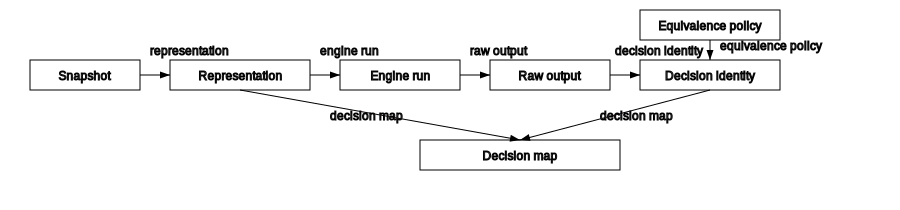
\includegraphics[width=\linewidth]{../../2026-01-31/agents/work-tree/figures/figure1_canonical_schematic.pdf}
\caption{Canonical decision-valued mapping schematic. A fixed snapshot is encoded into a representation family. Each representation is executed by a fixed engine and yields raw output. An equivalence policy extracts a discrete decision identity from the raw output. The decision map links representation identifiers, engine runs, and decision identities.}
\label{fig:canonical-decision-map}
\end{figure}

\begin{figure}[t]
\centering
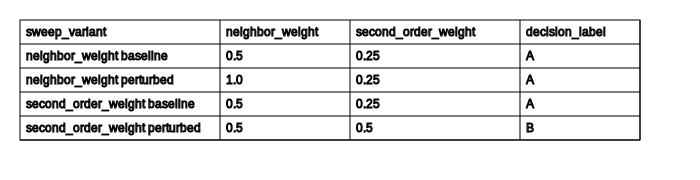
\includegraphics[width=\linewidth]{../../2026-01-31/agents/work-tree/figures/figure2_primary_sweep.pdf}
\caption{Primary representational sweep for one snapshot and engine. Each variant corresponds to a weight setting recorded in the weight variation results. Decision identity is defined by the route node sequence in each variant. Identical identities use the same label.}
\label{fig:primary-representational-sweep}
\end{figure}

\begin{figure}[t]
\centering
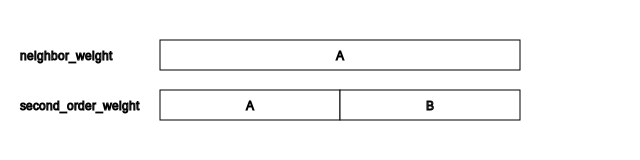
\includegraphics[width=\linewidth]{../../2026-01-31/agents/work-tree/figures/figure3_identity_persistence.pdf}
\caption{Identity persistence regions derived from Figure 2. Consecutive variants with identical decision identity labels are shown as a single region, indicating persistence under the tested weight changes.}
\label{fig:identity-persistence}
\end{figure}

\begin{figure}[t]
\centering
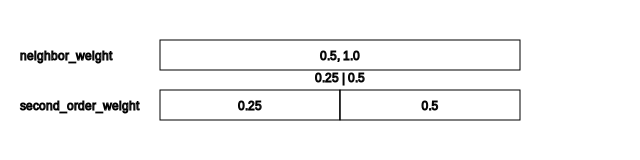
\includegraphics[width=\linewidth]{../../2026-01-31/agents/work-tree/figures/figure4_boundary_fracture.pdf}
\caption{Boundary and fracture localization derived from Figure 2. Transitions where route\_changed or edge\_order\_changed is true are marked as boundaries, with baseline and perturbed weight values listed.}
\label{fig:boundary-fracture}
\end{figure}

\begin{figure}[t]
\centering
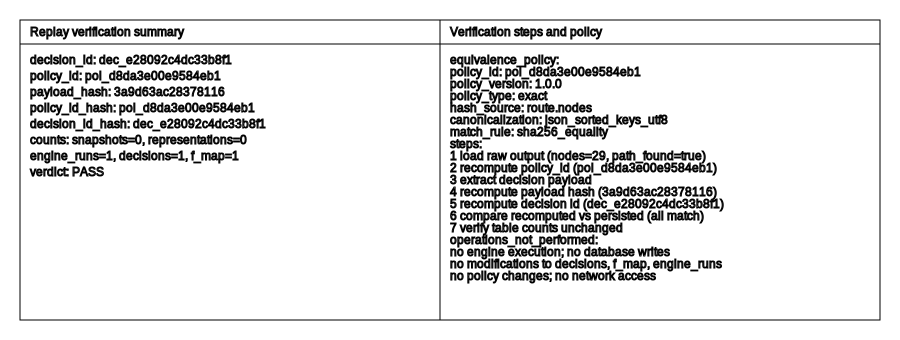
\includegraphics[width=\linewidth]{../../2026-01-31/agents/work-tree/figures/figure5_replay_verification.pdf}
\caption{Reproducibility replay verification. The replay verification logs show recomputed policy identifier, payload hash, and decision identifier matching the persisted manifest, and table counts remain unchanged.}
\label{fig:replay-verification}
\end{figure}

All figures will use the canonical caption template defined at the end of this manuscript. No figure will introduce performance metrics, optimization criteria, or learning claims.


% ------------------------------------------------------------------
% CANONICAL FIGURE CAPTION TEMPLATE (MANDATORY)
% All figures in this manuscript MUST use this caption structure.
% Any mention of performance, accuracy, loss, optimization, learning,
% or intelligence is a violation of manuscript scope.
%
% \textbf{Figure X:} Canonical representational sweep for a fixed snapshot and engine.
% Each point corresponds to a deterministic representation drawn from the declared
% representation family. Axes denote representation parameters. Color encodes discrete
% decision identity as defined by the equivalence policy. Contiguous regions indicate
% identity persistence; boundaries indicate identity change induced by representational
% variation.
% ------------------------------------------------------------------

\bibliographystyle{plain}
\bibliography{bibliography}

\end{document}
